% 第 6 章 — GPU 体系结构、CUDA 编程与最大化占用率（完全汉化版）
% 与 chapter06-presentation.pdf 逐页一一对应（52 页），可左右对照阅读。
% 编译：xelatex chapter06-presentation-zh.tex（跑两遍）
\documentclass[aspectratio=169]{beamer}

% ====== 演讲人信息 ======
\newcommand{\PresenterName}{Tianqin Cai}
\newcommand{\PresenterTitle}{Applied Scientist}
\newcommand{\PresenterOrg}{AWS}
% ========================

\usetheme{Madrid}
\definecolor{navy}{RGB}{18,47,90}
\definecolor{kwblue}{RGB}{0,56,132}
\definecolor{okgreen}{RGB}{80,130,20}
\usecolortheme[named=navy]{structure}
\setbeamercolor{frametitle}{bg=navy,fg=white}
\setbeamercolor{title}{bg=navy,fg=white}
\setbeamercolor{block title}{bg=navy,fg=white}
\setbeamercolor{block body}{bg=gray!12,fg=black}
\setbeamercolor{block title example}{bg=okgreen,fg=white}
\setbeamercolor{block body example}{bg=okgreen!10,fg=black}
\setbeamertemplate{navigation symbols}{}
\setbeamertemplate{blocks}[rounded][shadow=true]

% ---- 中文支持（xelatex + xeCJK）----
\usepackage{xeCJK}
\setCJKmainfont{Noto Sans CJK SC}
\setCJKsansfont{Noto Sans CJK SC}
\setCJKmonofont{Noto Sans CJK SC}
\XeTeXlinebreaklocale "zh"
\XeTeXlinebreakskip = 0pt plus 1pt

\usepackage{booktabs}
\usepackage{listings}
\lstset{
  language=C++,
  basicstyle=\ttfamily\fontsize{6.5}{7.6}\selectfont,
  keywordstyle=\color{kwblue}\bfseries,
  commentstyle=\color{gray}\itshape,
  stringstyle=\color{okgreen},
  showstringspaces=false,
  breaklines=true,
  columns=fullflexible
}

\newcommand{\kw}[1]{\textbf{\textcolor{kwblue}{#1}}}
\newcommand{\pe}[1]{{\footnotesize\itshape 大白话：#1}}
\newcommand{\refmark}[1]{\textsuperscript{[#1]}}

\title[AI Systems Performance Engineering]{AI Systems Performance Engineering}
\subtitle{第 6 章 —— GPU 体系结构、CUDA 编程与最大化占用率（Occupancy）}
\author[\PresenterName\ \ \PresenterTitle\ \ \PresenterOrg]{\PresenterName\\\PresenterTitle\\\PresenterOrg}
\institute[]{\footnotesize 面向应用科学家的 AI 基础设施内部培训}
\date{2026 年 8 月 15 日}

\begin{document}

% ================================================================ 1
\begin{frame}
  \titlepage
\end{frame}

% ================================================================ 2
\begin{frame}{这次讲什么 —— 以及为什么值得讲}
  \begin{block}{大白话版}
    GPU 是一台\kw{吞吐量机器}：它同时跑\kw{成千上万个线程}，靠"手头永远有别的活可干"来掩盖慢速内存。
    本章教你三样东西：\kw{词汇表}（warp、block、grid、SM）、\kw{内存阶梯}（寄存器 $\to$ 共享内存 $\to$ L2 $\to$ HBM），
    以及\kw{一条黄金法则}：发射足够多的并行工作，让每个 SM 都忙起来。
  \end{block}
  \begin{columns}[t]
    \column{0.48\textwidth}
    \begin{itemize}
      \item \kw{问题所在：}SM 闲着的 GPU 就是一台昂贵的取暖器 —— 大多数朴素写法的 kernel
            只用到硬件的百分之几。
      \item \kw{工具：}CUDA 的线程层级把你的算法映射到硬件上，且跨 GPU 代际\kw{无需改动}。
    \end{itemize}
    \column{0.48\textwidth}
    \begin{itemize}
      \item \kw{度量：}\emph{占用率（occupancy）}—— 在飞行中的 warp 数量占硬件上限的比例。
      \item \kw{指南针：}\emph{屋顶线模型（roofline）}在你动手优化之前，先告诉你 kernel
            是算力受限还是内存受限 —— 别修错了地方。
    \end{itemize}
  \end{columns}
  \medskip
  \centering\footnotesize\itshape
  本章是第 7--12 章一切 kernel 级内容的地基。
\end{frame}

% ================================================================ 3
\begin{frame}{路线图：五个部分，一条黄金法则}
  \begin{enumerate}
    \item \kw{GPU 体系结构}（第 4--19 页）—— 线程/block/grid、warp 与 SIMT、
          SM 内部（+ 车间比喻）、分化（divergence）、硬件上限、兼容性
    \item \kw{CUDA 编程}（20--27）—— kernel 解剖、启动参数、2D/3D 网格、异步内存分配
    \item \kw{内存层级}（28--36）—— 寄存器、共享内存/L1、TMEM、常量内存、L2、HBM3e、统一内存
    \item \kw{占用率实战}（37--45）—— 一个 22$\times$ 的案例、launch bounds、Occupancy API
    \item \kw{正确性与屋顶线}（46--49）—— Compute Sanitizer；算力受限 vs.\ 内存受限
  \end{enumerate}
  \medskip
  \pe{先让 GPU 忙起来，再让每个时钟周期都有产出；永远用 profiler 来判断该用哪种药方。}
\end{frame}

% ================================================================ 4
\begin{frame}{第一部分 —— GPU 优化吞吐量；CPU 优化延迟}
  \begin{columns}[c]
    \column{0.55\textwidth}
    \begin{itemize}
      \item CPU：核少、缓存深、\emph{单线程}快。GPU：数百个 \kw{SM}
            （流式多处理器，streaming multiprocessor）并行跑\kw{成千上万个线程}。
      \item 基本 CUDA 流程（右图）：主机把数据 \kw{CPU $\to$ GPU} 拷过去，启动一个 \kw{kernel}，
            再把结果拷回来。
      \item GPU 的答案不是"拷得更快"，而是\kw{海量并行}：
            一批线程在等内存时，另一批线程在干活。
      \item 甜区：\kw{数据并行}型工作 —— 矩阵乘、卷积 ——
            用 CUDA C++ 写，或经由 \kw{PyTorch} / OpenAI \kw{Triton} 间接写。\refmark{1,3}
    \end{itemize}
    \column{0.42\textwidth}
    \centering
    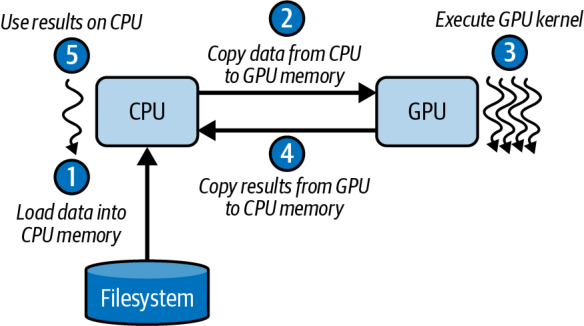
\includegraphics[width=\linewidth]{figs/fig6-1.png}\\
    {\scriptsize 图 6-1：最简单的 CUDA 编程流程}
  \end{columns}
  \medskip
  \pe{CPU 是跑车，GPU 是货运列车 —— 对列车的要求是\emph{装满}，不是跑得快。}
\end{frame}

% ================================================================ 5
\begin{frame}{线程层级：线程 $\to$ 线程块 $\to$ 网格}
  \begin{columns}[c]
    \column{0.52\textwidth}
    \begin{itemize}
      \item \kw{线程（thread）}：在一个数据元素上执行你的 kernel 代码。
      \item \kw{线程块（thread block，又叫 CTA：协作线程数组）}：最多 \kw{1{,}024 个线程}；
            共享片上高速的\kw{共享内存}。
      \item \kw{网格（grid）}：一次启动的全部 block —— 尺寸设对了，
            可以零改动地扩展到\kw{数百万线程}。
      \item CUDA 运行时（以及 PyTorch）负责把 block 调度、分发到所有 SM 上。
    \end{itemize}
    \column{0.45\textwidth}
    \centering
    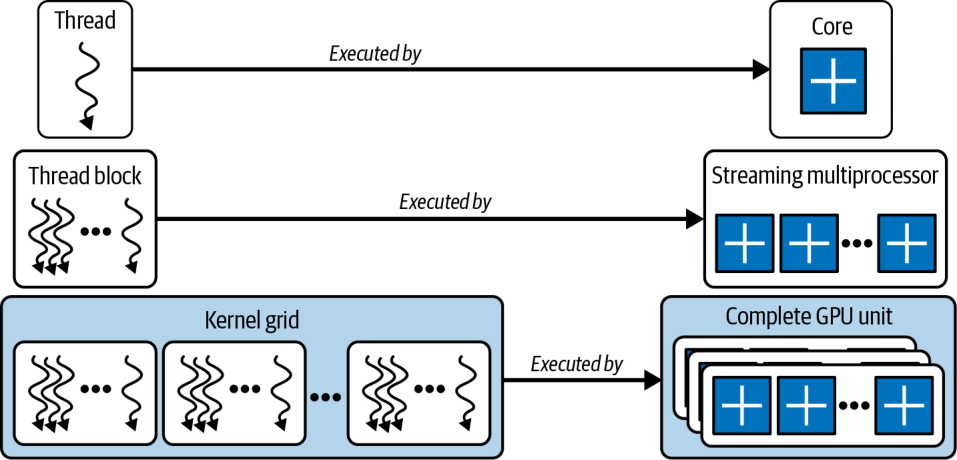
\includegraphics[width=\linewidth]{figs/fig6-3.png}\\
    {\scriptsize 图 6-3：线程、线程块（CTA）与网格}
  \end{columns}
  \medskip
  \pe{工人（线程）组成小队（block），队内沟通便宜；公司（grid）按活儿的大小招足够多的小队。}
\end{frame}

% ================================================================ 6
\begin{frame}{Warp 与 SIMT：32 个线程齐步走}
  \begin{columns}[c]
    \column{0.52\textwidth}
    \begin{itemize}
      \item block 被进一步切成\kw{每 32 个线程一组的 warp}，在 \kw{SIMT}
            （单指令多线程）模式下一起执行同一条指令。
      \item \kw{硬件真正调度的单位是 warp}，不是线程；
            warp 大小在\kw{每一代 GPU 上都是 32}。
      \item 硬件靠\kw{在 warp 之间快速切换}来掩盖长延迟事件
            （全局内存加载、缓存填充、流水线停顿）。
    \end{itemize}
    \column{0.45\textwidth}
    \centering
    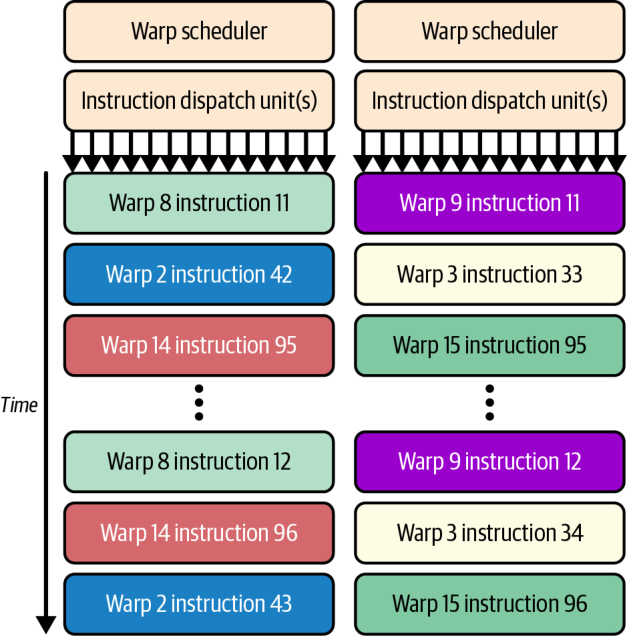
\includegraphics[width=0.8\linewidth]{figs/fig6-7.png}\\
    {\scriptsize 图 6-7：在 warp 调度器的指挥下，warp 作为整体向前推进}
  \end{columns}
  \medskip
  \pe{一个 warp 就是一支 32 人的赛艇队 —— 同一桨、同一拍，否则全船等着。}
\end{frame}

% ================================================================ 7
\begin{frame}{Blackwell SM 内部：资源预算}
  \begin{columns}[c]
    \column{0.52\textwidth}
    \begin{itemize}
      \item 每个 SM 最多同时追踪 \kw{64 个 warp} = \kw{2{,}048 个线程} ——
            这就是调度器来回切换的"待命池"。
      \item 每 SM 有 \kw{64K 个 32 位寄存器}（共 256 KB）；单个线程最多用 \kw{255 个}。
      \item \kw{256 KB} 的 L1 缓存 / 共享内存合并空间；最多 \kw{228 KB} 可配置为
            用户管理的共享内存（\kw{实际可用 227 KB} —— CUDA 每 block 保留 1 KB）。
      \item 正是这些片上预算，让一个 SM 能同时"抛接"几千个线程而不用频繁碰 DRAM。\refmark{2}
    \end{itemize}
    \column{0.45\textwidth}
    \centering
    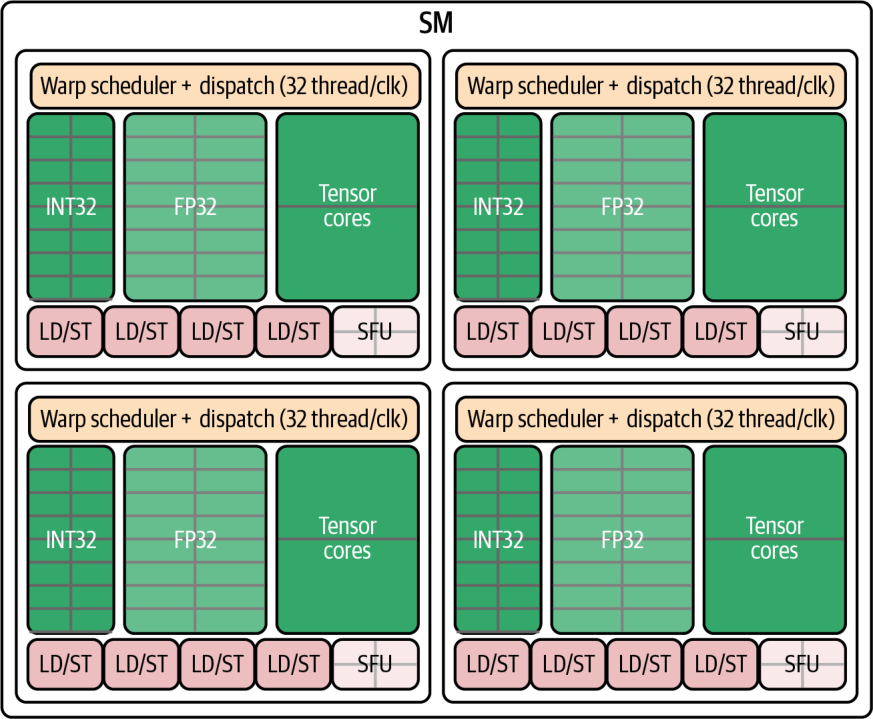
\includegraphics[width=0.8\linewidth]{figs/fig6-2.png}\\
    {\scriptsize 图 6-2：Blackwell SM —— 四个调度分区共享片上资源}
  \end{columns}
  \medskip
  \pe{SM 是一间车间：寄存器是每人的工具腰带，共享内存是公共工作台。}
\end{frame}

% ================================================================ 8
\begin{frame}{比喻：一个 SM 就是一间车间}
  \begin{columns}[c]
    \column{0.54\textwidth}
    \centering
    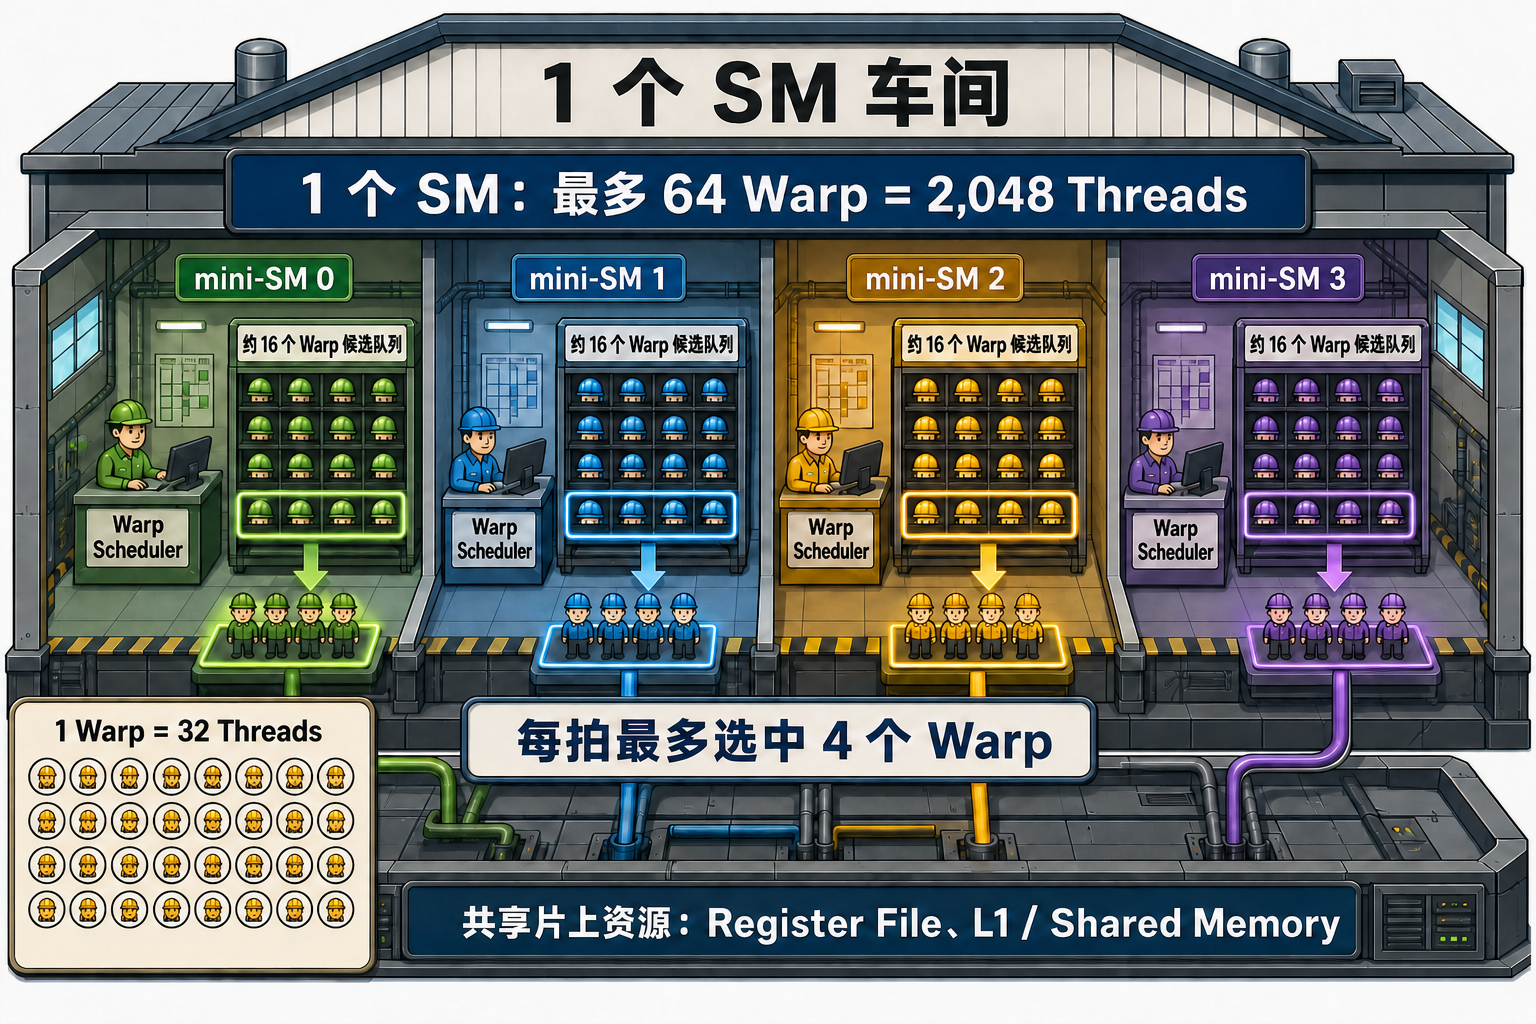
\includegraphics[width=\linewidth]{figs/analogy-sm-workshop.png}\\
    {\scriptsize 演讲人自制比喻图（非书中原图）}
    \column{0.44\textwidth}
    \begin{itemize}\footnotesize
      \item 四个彩色隔间 = SM 的 \kw{4 个调度分区}（"mini-SM"），
            各配一名 \kw{warp 调度器}（调度员）。\kw{不是} 4 个独立的 SM ——
            CUDA 眼里永远只有整个 SM。
      \item 货架上的安全帽 = \kw{常驻 warp}：每个分区约 16 个候选，
            \kw{共 64 个}。常驻 = 状态/寄存器已经分配好 ——
            \emph{不等于}"此刻正在执行"。
      \item 高亮的工人小组 = \kw{本拍被发射的 $\leq$4 个 warp}
            （每个调度员每拍最多挑 1 个\emph{就绪的} warp）。
      \item 左下角：\kw{1 个 warp = 32 个线程} —— 整组一起派工。
      \item 共同的地基：\kw{寄存器堆、L1、共享内存} ——
            还是同一个 SM 的资源，四个分区共用。
    \end{itemize}
  \end{columns}
  \smallskip
  \pe{64 支候选队伍待命，4 名调度员，每拍最多派出 4 支 —— 每支队伍 32 名工人。}
\end{frame}

% ================================================================ 9
\begin{frame}{让车间动起来：逐拍看延迟隐藏}
  \begin{columns}[t]
    \column{0.48\textwidth}
    \begin{block}{某个分区的某一瞬间}
      \small
      Warp A —— \kw{在等} HBM 的数据\\
      Warp B —— \kw{在等}上一条计算结果\\
      Warp C —— \kw{就绪}\qquad Warp D —— \kw{就绪}\\[4pt]
      调度员跳过 A 和 B，\kw{发射 C 或 D} ——
      跳过一个停顿的 warp \kw{不花任何代价}。
    \end{block}
    {\small
    \begin{tabular}{@{}ll@{}}
      \toprule
      \textbf{周期} & \textbf{被发射（举例）} \\
      \midrule
      1 & Warp C \\
      2 & Warp F \\
      3 & Warp D \\
      4 & Warp H \\
      \bottomrule
    \end{tabular}}
    \column{0.48\textwidth}
    \begin{itemize}
      \item "发射" = 这条指令\kw{开始执行}；不代表这一拍就能执行完。
      \item 延迟隐藏\kw{并没有}缩短任何 warp 的等待 ——
            它是\kw{用别的 warp 的工作把等待填满}。
      \item 这就是 \kw{64 个常驻 warp} 的意义：给 4 名调度员准备
            足够深的\emph{就绪}候选池 —— 也解释了低占用率为什么伤性能
            （没有可切换的对象）。
    \end{itemize}
  \end{columns}
  \medskip
  \pe{调度员从不站着干瞪打盹的队伍 —— 总有另一支队伍的零件已经到货了。}
\end{frame}

% ================================================================ 10
\begin{frame}{同一台机器的两套视角：软件 vs.\ 硬件}
  \begin{columns}[c]
    \column{0.56\textwidth}
    {\footnotesize\setlength{\tabcolsep}{3.5pt}
    \begin{tabular}{@{}lll@{}}
      \toprule
      \textbf{软件（你写的）} & \textbf{硬件（实际跑的）} & \textbf{比喻} \\
      \midrule
      Grid（网格） & 整块 GPU & 整座工厂 \\
      Block（线程块） & 恰好\kw{一个 SM} & 一间车间 \\
      \emph{（warp：隐式）} & 硬件调度的单位 & 32 人小组 \\
      Thread（线程） & warp 里的一条通道 & 一名工人 \\
      \bottomrule
    \end{tabular}}\\[6pt]
    \begin{itemize}\small
      \item 你决定 \kw{grid 和 block 的大小}；硬件决定
            \kw{block 放到哪个 SM、warp 何时被调度}。
      \item \kw{warp 是两套语言的桥}：硬件把每个 block 自动切成
            32 线程一组的 warp —— 全程对你透明。
      \item 内存预告（第三部分）：寄存器 = 随身工具箱，共享内存 = 公共工作台，
            L1 = 车间货架，\kw{L2 = 全厂中转仓}，\kw{HBM = 厂外大仓库}；
            一次全局读取依次尝试 L1 $\to$ L2 $\to$ HBM，数据原路返回。
    \end{itemize}
    \column{0.40\textwidth}
    \centering
    
\includegraphics[width=\linewidth]{figs/analogy-gpu-factory.png}\\
    {\scriptsize 演讲人自制比喻图：SM 车间、L2 中转仓、HBM 大仓库}
  \end{columns}
  \medskip
  \pe{软件说的是 grid 和 block；硬件回答的是 SM 和 warp —— warp 就是两套词汇表的交汇点。}
\end{frame}

% ================================================================ 11
\begin{frame}{四个 warp 调度器，双发射}
  \begin{columns}[c]
    \column{0.58\textwidth}
    \begin{itemize}
      \item 每个 SM = 四个"\kw{迷你 SM}"：相互独立的 warp 调度器，各自带取指/派发逻辑。
      \item 每个调度器每周期发射 \kw{1 条 warp 指令} $\Rightarrow$ 每周期最多
            \kw{4 个 warp 同时前进}。
      \item \kw{双发射（dual-issue）}：每周期可同时发 1 条数学指令（INT32/FP32/Tensor Core）
            \kw{+} 1 条访存指令（load/store）—— 但必须\emph{来自同一个 warp}，不能跨 warp 拼。
      \item 最好情况：每周期有 \kw{4 条数学 + 4 条访存}指令在飞。
    \end{itemize}
    \column{0.38\textwidth}
    \centering
    {\small
    \begin{tabular}{@{}ll@{}}
      \toprule
      \textbf{每周期（表 6-1）} & \textbf{上限} \\
      \midrule
      调度器数量 & 4 \\
      可发射 warp 数 & 4 \\
      数学 / 访存指令 & 4 / 4 \\
      \bottomrule
    \end{tabular}}\\[6pt]
    {\scriptsize 书中注：表中数值为示意；\\真实基准见本书 GitHub 仓库\refmark{7}}
  \end{columns}
  \medskip
  \pe{四条收银通道；每个收银员一手扫码（数学）、一手装袋（访存）。}
\end{frame}

% ================================================================ 12
\begin{frame}{SFU 与 Load/Store 流水线}
  \begin{columns}[t]
    \column{0.48\textwidth}
    \begin{block}{SFU —— 特殊函数单元}
      \begin{itemize}\small
        \item 负责\kw{超越函数}：正弦、余弦、倒数、平方根。
        \item 有\kw{自己独立的流水线} —— \emph{不}占用"数学+访存"双发射对。
        \item 慢函数永远不会堵住核心算力/访存管道 $\Rightarrow$
              混合运算的 kernel 获得更多\kw{指令级并行}。
      \end{itemize}
    \end{block}
    \column{0.48\textwidth}
    \begin{block}{LD/ST —— 加载/存储流水线}
      \begin{itemize}\small
        \item 每 SM 有 \kw{16 条 LD/ST 流水线}（每个调度器 4 条），
              服务 L1/共享内存、L2 与全局内存。
        \item \kw{注意（书中警告）：}具体数量与配对关系\kw{没有保证} ——
              请以 profiler 计数器和 \kw{Blackwell 调优指南}为准。\refmark{2}
      \end{itemize}
    \end{block}
  \end{columns}
  \medskip
  \pe{SFU 是商店后面的"疑难业务专柜"—— 复杂业务都去那儿办，快速通道就不会被堵住。}
\end{frame}

% ================================================================ 13
\begin{frame}{block 内部协作，block 之间独立}
  \begin{columns}[c]
    \column{0.52\textwidth}
    \begin{itemize}
      \item block 内部：通过共享内存交换数据，用
            \kw{\texttt{\_\_syncthreads()}} 同步（一个栅栏：所有人到齐才能继续）。
      \item \kw{每一次栅栏都要花时间} —— 书中的建议：\kw{尽量减少同步点}。
      \item block 之间：\kw{相互独立，不保证执行顺序}。正是这份自由让调度器可以把 block
            "撒"到所有 SM 上 —— 也让你的 kernel 在未来 SM 更多的 GPU 上\kw{不改一行地跑}。
    \end{itemize}
    \column{0.45\textwidth}
    \centering
    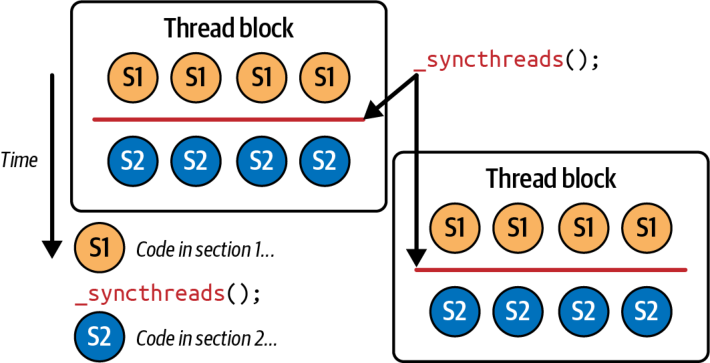
\includegraphics[width=0.9\linewidth]{figs/fig6-6.png}\\
    {\scriptsize 图 6-6：两段代码之间的 \texttt{\_\_syncthreads()}}
  \end{columns}
  \medskip
  \pe{小队碰头会（栅栏）有用但很贵 —— 能少开就少开；并且永远别假设 A 队比 B 队先干完。}
\end{frame}

% ================================================================ 14
\begin{frame}{线程块簇（Cluster）与 DSMEM}
  \begin{columns}[c]
    \column{0.52\textwidth}
    \begin{itemize}\small
      \item 传统上，\emph{不同} block 里的线程无法协作。现代 GPU 增加了
            \kw{线程块簇（thread block cluster）}：block 可以\kw{跨 SM} 通信，
            并有簇级的硬件栅栏。
      \item 底层支撑是 \kw{DSMEM}（分布式共享内存）：参与簇的各个 SM 的共享内存
            通过高速\kw{片上互连}拼成一个池子。
      \item 线程可以\kw{以片上速度}读、写、原子更新彼此的共享缓冲区
            —— \kw{完全不消耗全局内存带宽}。
      \item 这是 LLM 中超大矩阵乘的关键使能技术 —— 细节见\kw{第 10 章}。
    \end{itemize}
    \column{0.45\textwidth}
    \centering
    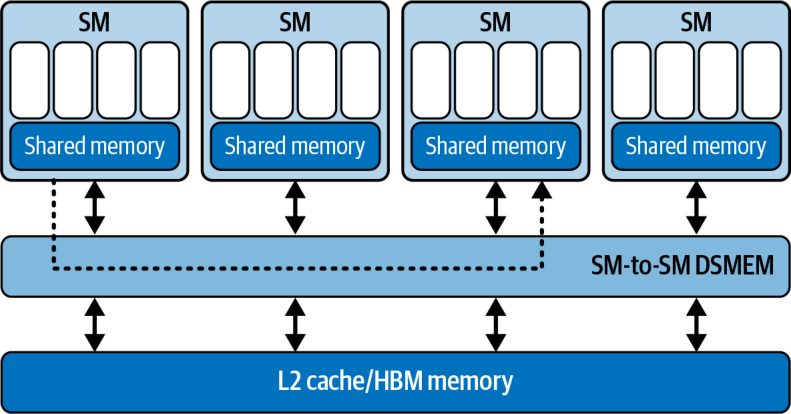
\includegraphics[width=\linewidth]{figs/fig6-5.png}\\
    {\scriptsize 图 6-5：簇内各 block 共享的 DSMEM}
  \end{columns}
  \medskip
  \pe{相邻小队在工作台之间的墙上开了一扇门，直接递零件，不用再通过仓库寄快递。}
\end{frame}

% ================================================================ 15
\begin{frame}{占用率（Occupancy）：本章的核心度量}
  \begin{block}{定义}
    \kw{占用率} = 一个 SM 上活跃的 warp 数 $\div$ 硬件上限（Blackwell 上是 64）。
    "\kw{实测占用率（achieved occupancy）}"是实际测得的平均值，由 Nsight Compute 报告。
  \end{block}
  \begin{columns}[t]
    \column{0.48\textwidth}
    \begin{itemize}
      \item 占用率高 $\Rightarrow$ 一个 warp 因等内存而停顿时，总有另一个 warp 顶上
            $\Rightarrow$ \kw{延迟隐藏}。
      \item Blackwell 的大寄存器堆（64K/SM）让高占用率更容易达到。
    \end{itemize}
    \column{0.48\textwidth}
    \begin{itemize}
      \item 制衡因素：warp 们共享\kw{寄存器和共享内存}。塞得太满
            $\Rightarrow$ \kw{寄存器溢出（spill）}到慢速内存 —— 你亲手制造了新的停顿。
      \item 所以：占用率要\kw{和}寄存器/共享内存用量\kw{放在一起}分析。
    \end{itemize}
  \end{columns}
  \medskip
  \pe{占用率就是车间的"上座率"—— 空位浪费延迟隐藏的机会，但塞太满就没人有工具可用了。}
\end{frame}

% ================================================================ 16
\begin{frame}{Warp 分化：当 {\ttfamily if/else} 把赛艇队劈成两半}
  \begin{columns}[c]
    \column{0.52\textwidth}
    \begin{itemize}
      \item 如果\emph{同一个 warp 内}的线程走了不同分支，warp 就会\kw{串行化}：
            先带着\kw{屏蔽（mask）}掉的另一半跑 \texttt{if} 路径，再跑 \texttt{else} 路径。
      \item 执行时间按\kw{不同路径的数量}成倍增长。
      \item \kw{跨 warp 没有惩罚} —— 不同 warp 各走各的分支，完全免费。
      \item 实用推论：让分支条件按 \kw{warp 对齐}
            （\texttt{threadIdx.x / 32}），而不是按线程奇偶（\texttt{threadIdx.x \% 2}）。
      \item 检测与治理：第 8 章（Nsight Compute）。
    \end{itemize}
    \column{0.45\textwidth}
    \centering
    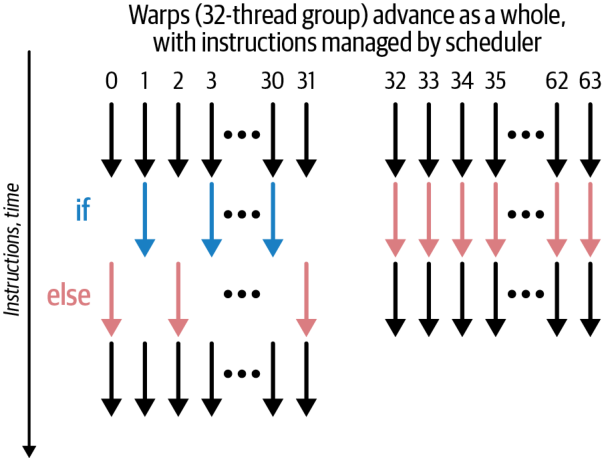
\includegraphics[width=0.85\linewidth]{figs/fig6-8.png}\\
    {\scriptsize 图 6-8：SIMT warp 分化（左）vs.\ 整齐一致（右）}
  \end{columns}
  \medskip
  \pe{赛艇队一半人往左划、一半人往右划，船就得把每个动作各做一遍 —— 慢一倍。}
\end{frame}

% ================================================================ 17
\begin{frame}{硬件上限 I：warp 与 block（表 6-2）}
  \begin{columns}[c]
    \column{0.52\textwidth}
    {\small
    \begin{tabular}{@{}ll@{}}
      \toprule
      \textbf{资源} & \textbf{上限（B200）} \\
      \midrule
      Warp 大小 & 32 线程 \\
      每 block 最大线程数 & 1{,}024 \\
      每 block 最大 warp 数 & 32 \ (= 1024 $\div$ 32) \\
      \bottomrule
    \end{tabular}}\\[6pt]
    {\scriptsize \texttt{blockDim.x $\times$ blockDim.y $\times$ blockDim.z $\leq$ 1024}}
    \column{0.45\textwidth}
    \begin{block}{为什么必须是 32 的倍数}
      \small 一个 \kw{33 线程的 block} 要占\kw{两个} warp 槽位 —— 第二个 warp 只有
      \kw{32 条通道中的 1 条}在干活，却占掉一个完整的调度槽。任何不是 32 倍数的设置，
      都在把调度能力白白捐给虚空。
    \end{block}
  \end{columns}
  \medskip
  \begin{itemize}
    \item block 太大 $\Rightarrow$ 每 block 需要太多寄存器 $\Rightarrow$ \kw{溢出（spill）}；
          或占太多共享内存（可用的 227 KB 由 SM 上\kw{所有常驻 block} 分摊）。
    \item block 小一点反而可能\kw{占用率更高} —— 每个 SM 能装下更多相互独立的 block。
  \end{itemize}
\end{frame}

% ================================================================ 18
\begin{frame}{硬件上限 II：SM 常驻与网格（表 6-3 / 6-4）}
  \begin{columns}[c]
    \column{0.55\textwidth}
    {\small\setlength{\tabcolsep}{4pt}
    \begin{tabular}{@{}ll@{}}
      \toprule
      \textbf{每 SM（常驻）} & \textbf{上限} \\
      \midrule
      最大 warp 数 & \kw{64}（= 2{,}048 线程） \\
      最大线程数 & 2{,}048 \\
      最大 block 数 & 32 \\
      \midrule
      \textbf{网格（grid）} & \\
      \midrule
      最大 block 数（X / Y / Z） & $\sim$21 亿 / 65{,}535 / 65{,}535 \\
      最大并发网格数 & 每设备 \kw{128} 个 kernel \\
      \bottomrule
    \end{tabular}}
    \column{0.42\textwidth}
    \centering
    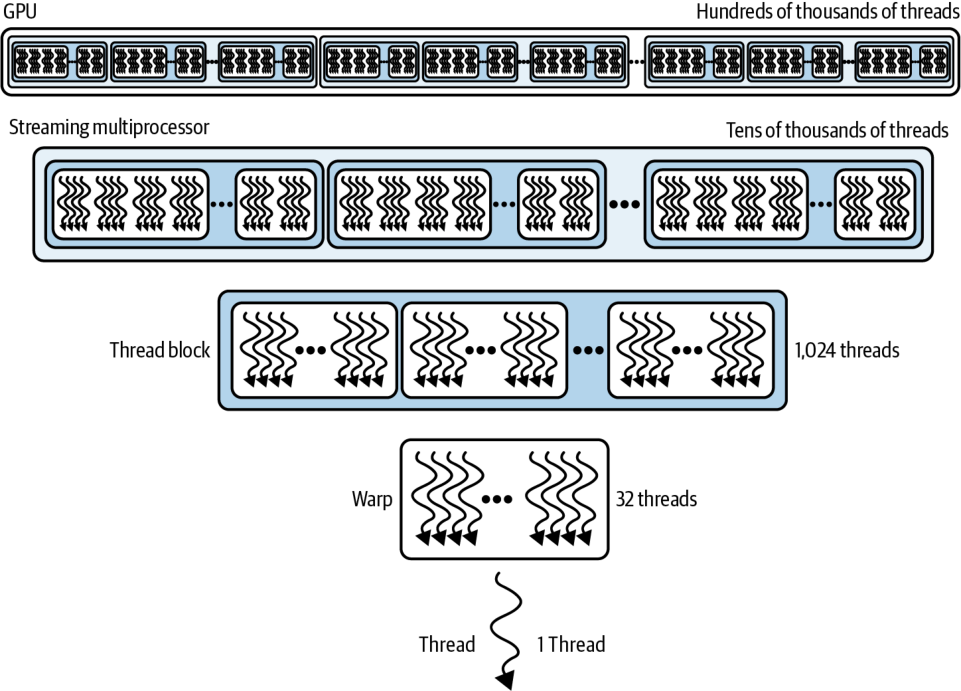
\includegraphics[width=\linewidth]{figs/fig6-9.png}\\
    {\scriptsize 图 6-9：各级线程资源的相对规模}
  \end{columns}
  \medskip
  \begin{itemize}\small
    \item 算例：block 取 1024 线程 $\Rightarrow$ 每 SM 只能放 \kw{2 个 block}；
          取 256 线程 $\Rightarrow$ \kw{8 个 block/SM} —— 同样是 2{,}048 线程，灵活性更高。
    \item 实践中你会先撞上\kw{每 SM 的上限}，远轮不到网格上限；
          Y/Z 方向 block 数超过 65{,}535 $\Rightarrow$ 改用 2D/3D 网格或多次启动。\refmark{1,2}
  \end{itemize}
\end{frame}

% ================================================================ 19
\begin{frame}{兼容性：PTX、SASS 与 Fatbin}
  \begin{columns}[t]
    \column{0.48\textwidth}
    \begin{itemize}
      \item \kw{SASS}：针对\emph{某一个}架构的最终机器码（sm\_90 = Hopper，
            sm\_100 = Blackwell）。只含 SASS 的二进制\kw{无法在更新的 GPU 上运行}。
      \item \kw{PTX}：虚拟指令集，由驱动在加载时 \kw{JIT 编译} $\Rightarrow$
            \kw{向前兼容}。
      \item 家族目标（\texttt{sm\_100f}）：可移植范围被限制在同一特性家族之内。
    \end{itemize}
    \column{0.48\textwidth}
    \begin{block}{最佳实践}
      \small 发布 \kw{fatbin}：通用 PTX \kw{+} 你需要深度优化的那些家族专用 cubin
      —— 并为其他架构准备\kw{回退路径}。
    \end{block}
    \begin{itemize}\small
      \item 用 \kw{\texttt{CUDA\_FORCE\_PTX\_JIT=1}} 验证：强制走 PTX JIT；
            如果二进制里没有 PTX，\kw{kernel 启动会直接失败} —— 那就得带上 PTX 重新构建。
    \end{itemize}
  \end{columns}
  \medskip
  \pe{PTX 是菜谱，SASS 是做好的菜 —— 把菜谱也一起发货，将来的厨房才能照着重做。}
\end{frame}

% ================================================================ 20
\begin{frame}[fragile]{第二部分 —— CUDA Kernel 解剖：设备侧}
  \begin{columns}[t]
    \column{0.52\textwidth}
\begin{lstlisting}
__global__ void myKernel(float* input, int N) {
    // unique global index for this thread
    int idx = blockIdx.x * blockDim.x + threadIdx.x;
    if (idx < N) {          // bounds check!
        input[idx] *= 2.0f; // in-place: double it
    }
}
\end{lstlisting}
    \begin{itemize}\small
      \item \kw{\texttt{\_\_global\_\_}}：在设备（GPU）上运行、可从主机（CPU）调用。
      \item 内置变量：\texttt{blockIdx}（我在哪个 block）、\texttt{blockDim}（block 多大）、
            \texttt{threadIdx}（我在 block 里排第几）。
    \end{itemize}
    \column{0.44\textwidth}
    \begin{itemize}
      \item kernel 是站在\kw{单个线程}的视角写的；
            \texttt{idx} 划出属于这个线程的那一小片数据。
      \item CUDA 把它编译成设备代码，由\kw{成千上万乃至上百万}个轻量线程并行执行。
      \item 启动语法（主机侧）：\kw{\texttt{<<<blocksPerGrid, threadsPerBlock>>>}} ——
            \emph{每一次} kernel 调用都绕不开的两个核心参数。
    \end{itemize}
  \end{columns}
  \medskip
  \pe{你只写\emph{一名}工人的岗位说明书；CUDA 复印一百万份，每份填上不同的行号。}
\end{frame}

% ================================================================ 21
\begin{frame}[fragile]{主机侧：六步数据流}
  \begin{columns}[t]
    \column{0.55\textwidth}
\begin{lstlisting}
const int N = 1'000'000;
float *h_input = nullptr, *d_input = nullptr;   // h_=host, d_=device
cudaMallocHost(&h_input, N * sizeof(float));    // 1) pinned host alloc
for (int i = 0; i < N; ++i) h_input[i] = 1.0f;  //    init
cudaMalloc(&d_input, N * sizeof(float));        //    device alloc
cudaMemcpy(d_input, h_input, N * sizeof(float),
           cudaMemcpyHostToDevice);             // 2) H2D copy
const int threadsPerBlock = 256;
const int blocksPerGrid =                       //    = 3,907 for 1M
    (N + threadsPerBlock - 1) / threadsPerBlock;
myKernel<<<blocksPerGrid, threadsPerBlock>>>(d_input, N); // 3) launch
cudaDeviceSynchronize();                        // 4) wait for device
cudaMemcpy(h_input, d_input, N * sizeof(float),
           cudaMemcpyDeviceToHost);             // 5) D2H copy
cudaFree(d_input); cudaFreeHost(h_input);       // 6) cleanup
\end{lstlisting}
    \column{0.42\textwidth}
    \begin{itemize}
      \item 命名惯例：\kw{\texttt{h\_}} = 主机指针，\kw{\texttt{d\_}} = 设备指针
            —— 全书通用。
      \item \kw{\texttt{cudaMallocHost}} = \kw{锁页（pinned）}内存 ——
            后面异步拷贝要想真正重叠，这是先决条件。
      \item 书中注：这个版本\emph{还没有充分优化} —— 它是一份简单而完整的\kw{模板}，
            全书后面都在改进它。
    \end{itemize}
  \end{columns}
\end{frame}

% ================================================================ 22
\begin{frame}{为什么要把 N 传进去？单线程视角}
  \begin{block}{书中的回答（意译）}
    CUDA kernel 函数被设计为\kw{在单个线程内部}工作，与成千上万个其他线程并肩，
    \kw{各自处理输入数据的一个分片}。因此 N 定义了这个 kernel 所要处理的分片边界。
  \end{block}
  \begin{itemize}
    \item CPU 函数可以自己查数组多长。kernel \kw{做不到} ——
          它拿到的只是一个裸指针，必须有人告诉它"世界的边界在哪"。
    \item N 与 \texttt{blockIdx}/\texttt{blockDim}/\texttt{threadIdx} 配合，
          让每个元素都被\kw{干净且不重不漏}地并行处理，横跨多个 SM。
    \item 这就是从 CPU 到 GPU 编程最核心的思维转变：你写的不是"处理这个数组"，
          而是"处理\kw{属于我的}那个元素 —— 如果它存在的话"。
  \end{itemize}
  \medskip
  \pe{一百万份复印的岗位说明书内容全一样；N 就是那行"活儿到哪里为止"。}
\end{frame}

% ================================================================ 23
\begin{frame}{边界检查 —— 以及错误的"延迟浮现"}
  \begin{columns}[t]
    \column{0.5\textwidth}
    \begin{block}{算例：N = 63}
      \small 调度器分配 \kw{2 个 warp}（64 线程）。warp 1 处理元素 0--31 —— 没问题。
      warp 2 处理 32--63，\kw{还多出一个线程}；没有 \texttt{if (idx < N)} 的话它就会读越界
      $\Rightarrow$ \kw{\texttt{cudaErrorIllegalAddress}}。
    \end{block}
    \begin{itemize}\small
      \item 书中规则：边界检查在 CUDA 代码里无处不在；"如果你没看到它，
            \kw{先搞清楚它为什么不在}。"
    \end{itemize}
    \column{0.47\textwidth}
    \begin{itemize}
      \item kernel \kw{异步执行，没有线程级异常}：一次非法访问只会给整个启动设置一个
            \kw{全局故障标志}。
      \item 主机要等到\kw{下一次同步或 CUDA API 调用}才能看到它 —— 错误是
            \kw{延迟浮现}的。
      \item 实践：启动后立刻
            \kw{\texttt{cudaGetLastError()} + \texttt{cudaDeviceSynchronize()}}，
            让故障在案发现场被抓住。
    \end{itemize}
  \end{columns}
  \medskip
  \pe{GPU 出事不会打电话给你 —— 它只留一张字条，你下次开信箱才看得到。}
\end{frame}

% ================================================================ 24
\begin{frame}{启动参数怎么选：256 配方}
  \begin{block}{几乎放之四海皆准的配方}
    先取 \kw{\texttt{threadsPerBlock = 256}}（8 个 warp）；
    \kw{\texttt{blocksPerGrid = (N + 255) / 256}}（向上取整 —— 每个元素都覆盖到）。
    再用 profiler 对比 128/512 微调。
  \end{block}
  \begin{itemize}
    \item \kw{32 的倍数}：没有半空的 warp 白占调度槽。
    \item \kw{延迟隐藏}：每 SM 几百个线程足以掩盖 DRAM 和指令停顿 ——
          8 block $\times$ 256 = 2{,}048，正好填满一个 SM，不多不少。
    \item \kw{占用率}：每 block 8 个 warp，通常寄存器和共享内存都能舒服地放下。
    \item \kw{资源均衡}：离 1{,}024 上限很远，又足够大到让 warp 一直有活干。
    \item 书中对 Blackwell 的提示：可以考虑每 block \kw{256--512} 线程。
  \end{itemize}
  \medskip
  \pe{256 是 block 大小里的"中杯咖啡"—— 第一次点单几乎不会错；profiler 说要改再改。}
\end{frame}

% ================================================================ 25
\begin{frame}[fragile]{2D 与 3D 的 kernel 输入}
  \begin{columns}[t]
    \column{0.52\textwidth}
\begin{lstlisting}
__global__ void my2DKernel(float* input,
                           int width, int height) {
    int x = blockIdx.x * blockDim.x + threadIdx.x;
    int y = blockIdx.y * blockDim.y + threadIdx.y;
    if (x < width && y < height) {  // 2D bounds check
        int idx = y * width + x;    // flatten to 1D
        input[idx] *= 2.0f;
    }
}
// host: dim3 threads(16,16);  // 256 threads, 2D
//       dim3 blocks((W+15)/16, (H+15)/16);
\end{lstlisting}
    \column{0.44\textwidth}
    \begin{itemize}
      \item 天生适合\kw{图像}：比如 $1{,}024 \times 1{,}024$ 的矩阵用
            $16 \times 16$ 的 block 处理（依然是 256 线程）。
      \item 同一套模式用 \kw{\texttt{dim3(x, y, z)}} 推广到 3D ——
            体数据直接映射到线程层级上。
      \item 书中注：本书大多数场景用 \kw{1D 或 2D（分块）}启动；
            纯 1D 时，普通 int 比 \texttt{dim3} 更顺手。
    \end{itemize}
  \end{columns}
  \medskip
  \pe{同一份菜谱，两个坐标轴：每个工人领到的是（行，列）工牌，而不是单个行号。}
\end{frame}

% ================================================================ 26
\begin{frame}[fragile]{异步分配内存：流（stream）与内存池}
  \begin{columns}[t]
    \column{0.52\textwidth}
\begin{lstlisting}
cudaStream_t s;
cudaStreamCreateWithFlags(&s, cudaStreamNonBlocking);

float* d_buf = nullptr;
cudaMallocAsync(&d_buf, N * sizeof(float), s);
myKernel<<<blocks, threads, 0, s>>>(d_buf, N);
cudaFreeAsync(d_buf, s);  // deferred until s finishes
\end{lstlisting}
    \begin{itemize}\small
      \item \kw{释放只等流 \texttt{s} 自己干完} —— 不做全局
            \texttt{cudaDeviceSynchronize}，也不跨流同步。
    \end{itemize}
    \column{0.45\textwidth}
    \begin{itemize}
      \item \texttt{cudaMalloc}/\texttt{cudaFree} 是\kw{同步且昂贵的}：
            全设备同步 + 操作系统调用（\texttt{mmap}/\texttt{ioctl}）、内核态上下文切换。
      \item \kw{\texttt{cudaMallocAsync}/\texttt{cudaFreeAsync}} 从每设备的
            \kw{内存池}里取：缓冲区循环利用、不跑操作系统、长训练循环下\kw{碎片更少}。
      \item 非阻塞流可避开老式\kw{默认流的隐式栅栏}（书中提示；多流重叠见第 11 章）。
    \end{itemize}
  \end{columns}
  \medskip
  \pe{在停车场常备一支车队，用时取钥匙 —— 别为每一单快递现买一辆车、送完再退掉。}
\end{frame}

% ================================================================ 27
\begin{frame}{调节内存池；PyTorch 的缓存分配器}
  \begin{columns}[t]
    \column{0.48\textwidth}
    \begin{block}{内存池的旋钮}
      \begin{itemize}\small
        \item \kw{\texttt{cudaMemPoolAttrReleaseThreshold}}（经
              \texttt{cudaMemPoolSetAttribute} 设置）：池子攒到多少保留内存才开始
              还给操作系统。
        \item \kw{\texttt{cudaMemPoolTrimTo}}：主动归还内存。
        \item 权衡：总\kw{占用量} vs.\ \kw{碎片化}。
      \end{itemize}
    \end{block}
    \column{0.48\textwidth}
    \begin{block}{与 PyTorch 的联系}
      \begin{itemize}\small
        \item PyTorch 的\kw{缓存分配器}（\texttt{PYTORCH\_ALLOC\_CONF}，旧名
              \texttt{PYTORCH\_CUDA\_ALLOC\_CONF}）就是同一个思想：复用 GPU 内存，
              避免每个迭代、每个新张量都同步调一次 \texttt{cudaMalloc}。
      \end{itemize}
    \end{block}
  \end{columns}
  \medskip
  \begin{itemize}
    \item 书中结论：一次性缓冲区 —— 用阻塞的 \texttt{cudaMalloc} 没问题；
          \kw{分配密集的循环 —— 异步 + 内存池}，性能更稳、吞吐更高。
  \end{itemize}
\end{frame}

% ================================================================ 28
\begin{frame}{第三部分 —— 内存阶梯一览}
  \begin{columns}[c]
    \column{0.58\textwidth}
    {\scriptsize\setlength{\tabcolsep}{2.5pt}
    \begin{tabular}{@{}lllll@{}}
      \toprule
      \textbf{层级} & \textbf{作用域} & \textbf{容量} & \textbf{延迟} & \textbf{带宽} \\
      \midrule
      寄存器 & 线程 & 256 KB / SM & $\sim$1 周期 & 数十 TB/s \\
      共享 + L1 & SM & 可用 228 KB & 20--30 周期 & TB 级 \\
      TMEM & SM & 256 KB (TC) & $\sim$10 周期 & TB 级 \\
      常量缓存 & SM & 8 / 64 KB & 1 周期广播 & TB 级 \\
      L2 缓存 & 全 GPU & \kw{126 MB} & $\sim$200 周期 & 数 TB/s \\
      本地（溢出区） & 线程 & 落在 DRAM & $\leq$1000 周期 & --- \\
      全局 HBM3e & 设备 & \kw{180 GB}（B200） & $\leq$1000 周期 & \kw{$\sim$8 TB/s} \\
      \bottomrule
    \end{tabular}}\\[4pt]
    {\scriptsize 表 6-5：每一级都在用容量换延迟/带宽。}
    \column{0.39\textwidth}
    \centering
    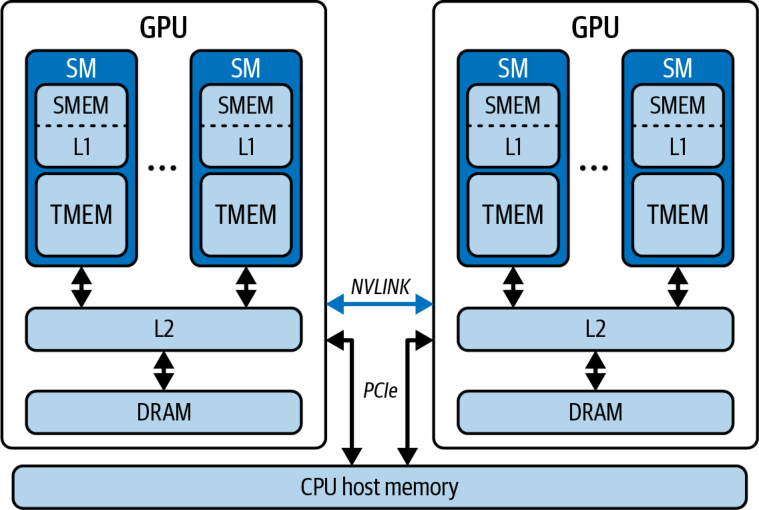
\includegraphics[width=\linewidth]{figs/fig6-10.png}\\
    {\scriptsize 图 6-10：GPU 内存层级（含 CPU 一侧）}
  \end{columns}
  \medskip
  \pe{书桌（寄存器）$\to$ 办公室书架（共享内存）$\to$ 楼里的图书馆（L2）$\to$ 城另一头的仓库（HBM）。活儿要在书桌上干。}
\end{frame}

% ================================================================ 29
\begin{frame}{寄存器 —— 以及"溢出悬崖"}
  \begin{columns}[c]
    \column{0.55\textwidth}
    \begin{itemize}
      \item 每个线程的数据之旅都从\kw{寄存器堆}出发：单周期读写，
            几乎不与任何人抢 —— 每 SM \kw{数十 TB/s}。
      \item 预算：每 SM 64K 个寄存器，\kw{单线程最多 255 个}。
      \item 悬崖：需要的更多（局部变量太多、编译器临时量）$\Rightarrow$
            超出的部分\kw{溢出到本地内存（local memory）} —— 名字里带"本地"，
            实际住在\kw{片外 DRAM}：几百到 1000+ 周期。
      \item 盯住 Nsight Compute 里的 \kw{"Registers Per Thread"} ——
            溢出是无声的杀手。
    \end{itemize}
    \column{0.42\textwidth}
    \centering
    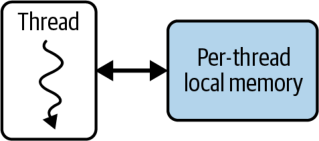
\includegraphics[width=0.6\linewidth]{figs/fig6-12.png}\\
    {\scriptsize 图 6-12：线程私有的本地内存（溢出区，落在 DRAM）}
  \end{columns}
  \medskip
  \pe{"本地内存"是城另一头的自助仓储柜，不是你的口袋。}
\end{frame}

% ================================================================ 30
\begin{frame}[fragile]{共享内存 + L1：一块 SRAM，两份工作}
  \begin{columns}[c]
    \column{0.55\textwidth}
    \begin{itemize}
      \item 每 SM 一块 \kw{256 KB 的 SRAM}，在用户管理的\kw{共享内存}
            （最多 228 KB；每 block 实际可用 227）和 \kw{L1/数据缓存}之间划分。
      \item \kw{划分比例（carveout）}由你选择：
    \end{itemize}
\begin{lstlisting}
cudaFuncSetAttribute(myKernel,
  cudaFuncAttributePreferredSharedMemoryCarveout,
  carveoutPercent);
\end{lstlisting}
    \begin{itemize}
      \item $\sim$20--30 周期；避开 \kw{bank 冲突}（多个线程撞上同一个存储 bank
            $\Rightarrow$ 访问被串行化）就能拿到 \kw{TB/s 级}带宽。
      \item 这就是\kw{block 内协作}的工作台 —— 分块（tile）、归约、数据中转都在这里。
    \end{itemize}
    \column{0.42\textwidth}
    \centering
    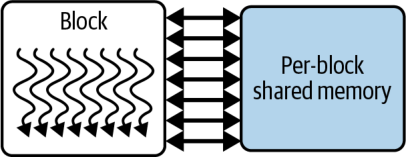
\includegraphics[width=0.75\linewidth]{figs/fig6-13.png}\\
    {\scriptsize 图 6-13：线程块的共享内存}
  \end{columns}
  \medskip
  \pe{一张工作台，隔板可调：多少留给团队的项目桌，多少留给自动整理的缓存架。}
\end{frame}

% ================================================================ 31
\begin{frame}{TMEM 与 TMA：给 Tensor Core 喂料}
  \begin{columns}[c]
    \column{0.55\textwidth}
    \begin{itemize}
      \item \kw{TMEM}：每 SM 专属的 \kw{256 KB SRAM}，是第五代 Tensor Core 指令
            （\texttt{tcgen05.*}、\kw{UMMA}）的\kw{累加器}；与 Tensor Core 之间数十 TB/s。
      \item 在 CUDA C++ 里\kw{不能用指针直接寻址} —— 数据搬运由
            \kw{TMA}（张量内存加速器）按\kw{描述符（descriptor）}编排。
      \item 以 $C = A \times B$ 为例：操作数 B 放 SMEM，A 和累加器放 TMEM；
            TMA 把分块沿 HBM $\to$ L2 $\to$ SMEM 搬运；SMEM $\leftrightarrow$ TMEM
            则由 Tensor Core 指令隐式完成。
      \item 净效果：\kw{大幅降低 Tensor Core 对全局内存的依赖}。细节见第 10 章。
    \end{itemize}
    \column{0.42\textwidth}
    \centering
    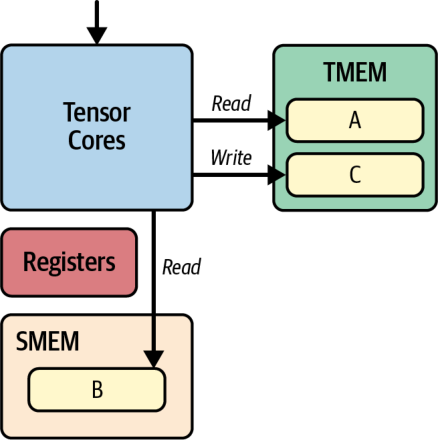
\includegraphics[width=0.72\linewidth]{figs/fig6-11.png}\\
    {\scriptsize 图 6-11：TMEM + SMEM 为 $C = A\times B$ 服务 Tensor Core}
  \end{columns}
  \medskip
  \pe{TMA 是在后台运货的叉车班组；大厨们从头到尾不用离开灶台。}
\end{frame}

% ================================================================ 32
\begin{frame}{常量缓存：单周期广播}
  \begin{columns}[t]
    \column{0.52\textwidth}
    \begin{itemize}
      \item 每 SM 约 \kw{8 KB 缓存}，服务 64 KB 的 \kw{\texttt{\_\_constant\_\_}} 空间。
      \item 超能力：当一个 warp 的 32 个线程全部读\kw{同一个地址}时，
            缓存\kw{单周期广播}这个值 —— 和读寄存器一样快。
      \item 各线程读不同地址则\kw{按通道串行化}；缓存未命中代价更高 —— 所以它适合
            \kw{小的、只读的、访问一致的}数据。
    \end{itemize}
    \column{0.45\textwidth}
    \begin{exampleblock}{书中给出的 LLM 例子}
      \begin{itemize}\small
        \item 旋转位置编码（RoPE）的查找表
        \item ALiBi 斜率
        \item LayerNorm 的 $\gamma$/$\beta$ 向量
        \item 嵌入量化的 scale 系数
      \end{itemize}
      \smallskip
      {\small 所有线程共享，\kw{全局内存流量为零}。}
    \end{exampleblock}
  \end{columns}
  \medskip
  \pe{它是喇叭，不是信箱：一次广播传到全部 32 名工人耳朵里 —— 前提是大家问的是同一个问题。}
\end{frame}

% ================================================================ 33
\begin{frame}{L2 缓存：全 GPU 的中间人}
  \begin{columns}[t]
    \column{0.52\textwidth}
    \begin{itemize}
      \item \kw{126 MB}，由所有 SM 共享 —— 连接片上 SRAM 与片外 HBM3e 的胶水层。
      \item $\sim$200 周期，聚合带宽\kw{数十 TB/s}；同时兜住 L1 放不下的部分。
      \item \kw{跨 block 复用}：一个 block 取过的数据，别的 block 可以直接用
            —— \kw{不必再去 DRAM 走一趟}。
    \end{itemize}
    \column{0.45\textwidth}
    \begin{block}{访存合并规则（书中提示）}
      \small 把全局内存加载组织成 \kw{128 字节对齐、可合并（coalesced）}的段，
      与缓存行整齐对应 —— 避免拆分事务，同时榨满 L2 \kw{和} DRAM 带宽。
      （具体怎么做：第 7 章。）
    \end{block}
  \end{columns}
  \medskip
  \pe{L2 是楼里的图书馆：同事已经从仓库借来的书，你直接在书架上拿 —— 前提是大家都按"整层书架"借，别一页一页地借。}
\end{frame}

% ================================================================ 34
\begin{frame}{全局 HBM3e、双芯粒 B200 与一致性}
  \begin{columns}[c]
    \column{0.55\textwidth}
    \begin{itemize}
      \item B200 上 \kw{180 GB}（B300 约 288 GB），带宽 \kw{$\sim$8 TB/s} —— 但延迟
            \kw{几百到 1000+ 周期}：整条链路上最慢的一环。
      \item 寄存器溢出、超大的自动数组（本地内存）也要付同样的代价。
      \item \kw{冷知识（书中注）}：B200 = \kw{两块光刻极限大小的裸片}用
            \kw{10 TB/s} 的片间互连拼起来，各带 4 个 HBM3e 栈 ——
            但呈现给你的是\kw{一块 GPU、一个地址空间}。
      \item \kw{一致性点（point of coherency，图 6-15）}：内存一致性按
            线程 $\to$ block $\to$ 簇 $\to$ 设备 $\to$ 系统的作用域逐级建立 ——
            通信范围越广，代价越高。
    \end{itemize}
    \column{0.42\textwidth}
    \centering
    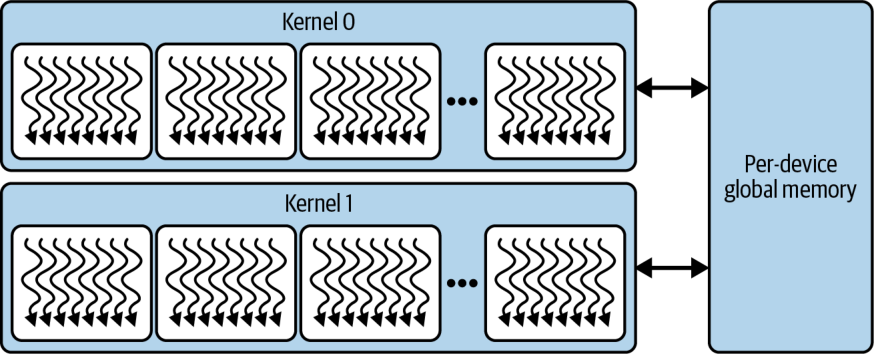
\includegraphics[width=\linewidth]{figs/fig6-14.png}\\[2pt]
    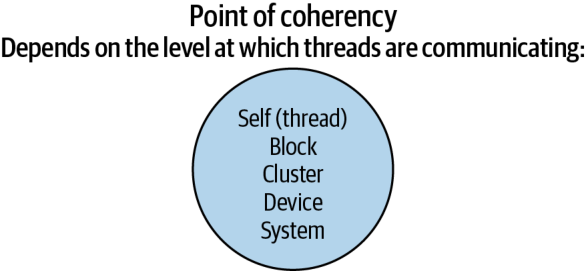
\includegraphics[width=0.9\linewidth]{figs/fig6-15.png}\\
    {\scriptsize 图 6-14 / 6-15：全局内存；各级一致性点}
  \end{columns}
\end{frame}

% ================================================================ 35
\begin{frame}{统一内存（Unified Memory）：方便，但有代价}
  \begin{columns}[c]
    \column{0.55\textwidth}
    \begin{itemize}
      \item \kw{\texttt{cudaMallocManaged()}}：CPU+GPU 一个连贯的地址空间 ——
            不用分开开两份缓冲区，也不用手写 \texttt{cudaMemcpy}。
      \item 底层机制：内存页在 CPU 和 GPU 之间的连接链路上\kw{按需迁移}。
      \item 代价：GPU 摸到一个还在 CPU 侧的页 $\Rightarrow$ \kw{缺页中断，kernel 停摆}。
      \item 走 PCIe 时：按需搬页可能\kw{比手动 memcpy 还慢}。
            在 Grace 超级芯片上，\kw{NVLink-C2C}（$\sim$900 GB/s）能让迁移接近
            本地速度 —— \kw{但延迟永远不为零}。
    \end{itemize}
    \column{0.42\textwidth}
    \centering
    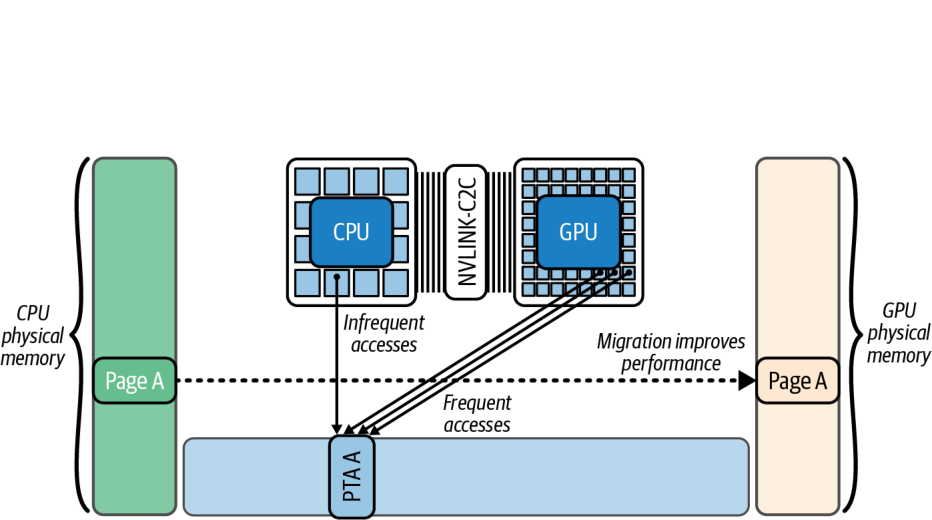
\includegraphics[width=\linewidth]{figs/fig6-16.png}\\
    {\scriptsize 图 6-16：统一内存的自动页迁移}
  \end{columns}
  \medskip
  \pe{统一内存是客房送餐：确实方便，但不提前点单，开饭（kernel 启动）时就得饿着等。}
\end{frame}

% ================================================================ 36
\begin{frame}[fragile]{驯服统一内存：预取、建议、绑定}
  \begin{columns}[t]
    \column{0.55\textwidth}
\begin{lstlisting}
// 1) move data BEFORE the kernel needs it:
cudaMemPrefetchAsync(ptr, size, gpuId, s);
// 2) tell the driver how you'll use it:
cudaMemAdvise(ptr, size,
    cudaMemAdviseSetPreferredLocation, gpuId);
cudaMemAdvise(ptr, size,
    cudaMemAdviseSetReadMostly, gpuId);
cudaMemAdvise(ptr, size,
    cudaMemAdviseSetAccessedBy, otherGpuId);
// 3) confine faults/migrations to one stream:
cudaStreamAttachMemAsync(stream, ptr, 0,
    cudaMemAttachSingle);
\end{lstlisting}
    \column{0.42\textwidth}
    \begin{itemize}\small
      \item \kw{预取（prefetch）}把"首次触碰才搬页"变成\kw{可重叠的异步传输}（图 6-17）。
      \item \kw{ReadMostly}：允许只读副本各处复制；\kw{AccessedBy}：让另一块 GPU
            直接映射页面而\kw{不}迁移（图 6-18）。
      \item \kw{Attach}：不让\emph{其他}流因为这段内存而停下来等。
      \item 没有 NVLink-C2C？把数据固定在 \kw{NUMA 本地}（对等拷贝/预取）。
      \item 结果：性能\kw{接近手动 \texttt{cudaMemcpy}}，简洁性照旧保留。
    \end{itemize}
  \end{columns}
\end{frame}

% ================================================================ 37
\begin{frame}{第四部分 —— 占用率的基本规则}
  \begin{block}{CUDA 性能第一基本法则（书中原则）}
    \centering \kw{"发射足够多的并行工作，把 GPU 填满。"}
  \end{block}
  \begin{columns}[t]
    \column{0.48\textwidth}
    \begin{block}{规则 1 —— 占用率低，性能差}
      \small 第一味药：\kw{增加并行度}（更多 block/线程），直到占用率在现代 GPU 上
      接近 \kw{80--100\%}。
    \end{block}
    \column{0.48\textwidth}
    \begin{block}{规则 2 —— 占用率已经很高}
      \small 如果 kernel 是\kw{内存受限}的，硬推到 100\% 没有用：你只需要
      \kw{"刚好够隐藏延迟"的 warp 数} —— 超过之后，瓶颈是带宽。
    \end{block}
  \end{columns}
  \medskip
  \begin{itemize}
    \item 接下来：同一个运算（$C = A + B$，$N = 10^6$），两种实现，
          以及 profiler 分别怎么评价它们。
  \end{itemize}
  \medskip
  \pe{规则 1 是把座位坐满；规则 2 提醒你：坐满的公交车堵在路上，照样动不了。}
\end{frame}

% ================================================================ 38
\begin{frame}[fragile]{案例第 1 回合：addSequential}
  \begin{columns}[t]
    \column{0.52\textwidth}
\begin{lstlisting}
// Single thread does ALL N additions
__global__ void addSequential(const float* A,
    const float* B, float* C, int N) {
  if (blockIdx.x == 0 && threadIdx.x == 0) {
    for (int i = 0; i < N; ++i) {
      C[i] = A[i] + B[i];
    }
  }
}
// Note: this kernel assumes <<<1,1>>>.
addSequential<<<1,1>>>(d_A, d_B, d_C, N);
cudaDeviceSynchronize();
\end{lstlisting}
    \column{0.44\textwidth}
    \begin{itemize}
      \item 一个线程、一个 warp、一个 SM —— \kw{其余全体围观}。
      \item 书中评语（意译）：GPU 庞大的资源基本闲置……占用率极差，性能自然极低。
      \item 没有其他 warp 可切换 $\Rightarrow$ 等内存的时间全部变成
            \kw{纯粹的空转} —— 延迟隐藏为零。
    \end{itemize}
  \end{columns}
  \medskip
  \pe{你租下了整座工厂，然后只雇了一名工人。}
\end{frame}

% ================================================================ 39
\begin{frame}[fragile]{同一个坑的 PyTorch 版}
  \begin{columns}[t]
    \column{0.52\textwidth}
\begin{lstlisting}[language=Python]
import torch
N = 1_000_000
A = torch.arange(N, dtype=torch.float32,
                 device='cuda')
B = 2 * A
C = torch.empty_like(A)
torch.cuda.synchronize()
# Naive, sequential GPU ops - DO NOT DO THIS
with torch.inference_mode():
    for i in range(N):     # N tiny serial kernels!
        C[i] = A[i] + B[i]
torch.cuda.synchronize()
\end{lstlisting}
    \column{0.44\textwidth}
    \begin{itemize}
      \item 用 Python 循环套 GPU 操作，等于\kw{串行发射 N 个迷你 kernel} ——
            GPU 沦为"一个标量的、毫无并行的处理器"。
      \item 占用率一样惨不忍睹，还要外加 \kw{每次启动的 CPU 开销} $\times$ 1{,}000{,}000。
      \item 书中建议：几乎总能找到\kw{PyTorch 原生的向量化实现}
            —— 包括编译器自动生成的版本。
    \end{itemize}
  \end{columns}
  \medskip
  \pe{最常见的 GPU 性能 bug：一不小心把 GPU 当成了一颗非常昂贵的单核 CPU 在用。}
\end{frame}

% ================================================================ 40
\begin{frame}[fragile]{案例第 2 回合：addParallel —— 以及 \texttt{C = A + B}}
  \begin{columns}[t]
    \column{0.52\textwidth}
\begin{lstlisting}
// One thread per element
__global__ void addParallel(
    const float* __restrict__ A,
    const float* __restrict__ B,
    float* __restrict__ C, int N) {
  int idx = blockIdx.x*blockDim.x + threadIdx.x;
  if (idx < N) C[idx] = A[idx] + B[idx];
}
addParallel<<<(N+255)/256, 256>>>(dA, dB, dC, N);
\end{lstlisting}
    {\small 书中的完整版本还用了锁页主机内存、非阻塞流和
    \texttt{cudaMallocAsync}/\texttt{cudaMemcpyAsync} —— 正是第二部分养成的习惯。}
    \column{0.44\textwidth}
    \begin{itemize}
      \item 约 3{,}907 个 block $\times$ 256 线程 —— \kw{一百万个线程}铺满整个数组
            （图 6-19）。
      \item \kw{\texttt{\_\_restrict\_\_}}：承诺指针互不重叠（无别名）——
            解开编译器优化的手脚。
      \item PyTorch 等价写法只有一行：\kw{\texttt{C = A + B}} ——
            单个向量化 kernel，同时调动大量线程。
    \end{itemize}
  \end{columns}
  \medskip
  \pe{还是那座工厂，现在每个工位都有人 —— 而 PyTorch 版等于直接"找劳务公司包了"。}
\end{frame}

% ================================================================ 41
\begin{frame}[fragile]{怎么量：nsys 与 ncu}
  \begin{columns}[t]
    \column{0.55\textwidth}
\begin{lstlisting}[language=bash]
# Nsight Systems: whole-app timeline
nsys profile --stats=true -t cuda,nvtx \
     -o report ./add_parallel.py

# Nsight Compute: per-kernel counters
ncu --section SpeedOfLight \
    --metrics sm__warps_active.avg.\
pct_of_peak_sustained_active,gpu__time_duration.avg \
    --target-processes all \
    --print-summary per-gpu -o report ./add_parallel.py
\end{lstlisting}
    \column{0.42\textwidth}
    \begin{itemize}
      \item \kw{nsys} 回答"\kw{时间花到哪儿去了} —— GPU 是没喂饱还是被堵住了？"
      \item \kw{ncu} 回答"\kw{这个 kernel 为什么慢} —— 占用率？停顿？缓存未命中？"
      \item \kw{两个都要跑}：只跑 nsys 看不到 kernel 内部的低效；只跑 ncu
            看不出数据\kw{喂得够不够快}。
      \item 那个很长的 \texttt{sm\_\_warps\_active...} 指标\kw{就是}实测占用率。
    \end{itemize}
  \end{columns}
  \medskip
  \pe{nsys 是给整台机器计时的秒表；ncu 是对准单个 kernel 的显微镜。}
\end{frame}

% ================================================================ 42
\begin{frame}{结果：只靠占用率就拿到 22$\times$}
  \begin{columns}[c]
    \column{0.52\textwidth}
    {\small
    \begin{tabular}{@{}lrr@{}}
      \toprule
      \textbf{指标} & \textbf{串行版} & \textbf{并行版} \\
      \midrule
      Kernel 耗时（ms） & 48.21 & \kw{2.17} \\
      GPU 利用率 & 1.5\% & \kw{95\%} \\
      实测占用率 & 1.3\% & \kw{38.7\%} \\
      Warp 执行效率 & 3.1\% & \kw{100\%} \\
      \bottomrule
    \end{tabular}}\\[4pt]
    {\scriptsize 表 6-6（示意值 —— 真实基准见本书代码仓库\refmark{7}）。
    Warp 效率 3.1\% $\approx$ 1/32：每个 warp 只有一条通道在干活。}
    \column{0.45\textwidth}
    \centering
    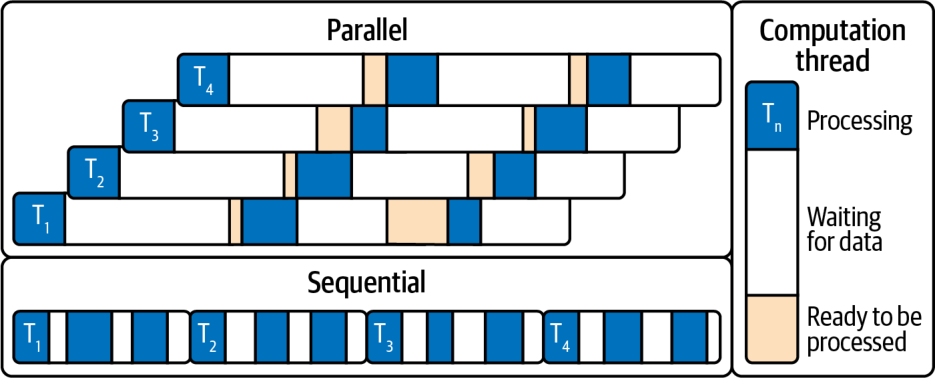
\includegraphics[width=\linewidth]{figs/fig6-20.png}\\
    {\scriptsize 图 6-20：串行版时间线上全是空档；并行版里其他 warp 的工作把空档填满了}
  \end{columns}
  \medskip
  \begin{itemize}\small
    \item 注意：38.7\% 的占用率就已经换来 22$\times$ —— 并不需要 100\%。
    \item 工具不同、名字不同：nsys 叫"GPU Utilization"，ncu 叫"SM Active \%" ——
          反映的都是 SM 被活跃 warp 占满的程度。
  \end{itemize}
\end{frame}

% ================================================================ 43
\begin{frame}{现实检验：内存受限的负载（LLM 解码）}
  \begin{itemize}
    \item 并行度拉满之后，下一个抓手是单 warp 效率（ILP 等，第 8 章）。但是：
          \kw{哪怕占用率 100\%}，只要 kernel 是\kw{内存受限}的 ——
          受制于数据搬运而非计算 —— 性能照样上不去。
    \item 书中的经典例子：\kw{LLM 的解码（decode）阶段} ——
          每生成一个 token，都要把\kw{模型权重}从 HBM 整个流进寄存器/共享内存。
    \item 几千亿参数 $\times$ 约 1 字节 $\approx$ 每趟\kw{几百 GB} ——
          不管你开多少线程，这都会\kw{把内存带宽打满}。
  \end{itemize}
  \begin{block}{让情况雪上加霜的趋势（书中注）}
    \kw{GPU 算力的增速超过了内存带宽。}Blackwell 的 HBM3e 约 8 TB/s，
    但算力和模型规模涨得更快 —— 在现代 AI 负载里，\kw{优化数据搬运是绝对关键}。
  \end{block}
  \medskip
  \pe{整个活儿就是"从仓库搬箱子"的话，前台多雇几个职员没有用 —— 屋顶线模型（第五部分）把这件事讲成了公式。}
\end{frame}

% ================================================================ 44
\begin{frame}[fragile]{\texttt{\_\_launch\_bounds\_\_}：编译期的占用率控制}
  \begin{columns}[t]
    \column{0.5\textwidth}
\begin{lstlisting}
// promise: never launched with > 256 thr/block
// request: keep >= 16 blocks resident per SM
__global__ __launch_bounds__(256, 16)
void myKernel(...) { /* ... */ }
\end{lstlisting}
    \begin{itemize}\small
      \item 16 $\times$ 256 = 4{,}096 $>$ 2{,}048 的上限 $\Rightarrow$ 编译器\kw{压回}
            8 个 block 并给出警告：\\
            {\scriptsize\texttt{ptxas warning: ... .minnctapersm will be ignored}}
    \end{itemize}
    \column{0.47\textwidth}
    \begin{itemize}
      \item 效果：编译器\kw{限制每线程寄存器数}（还可能收紧循环展开/内联），
            以避免溢出、让\kw{每个 SM 装下更多 warp}。
      \item 这笔交易：拿一点\kw{单线程性能}，换\kw{更稳定的 warp 吞吐}
            （更多 warp 在飞）。
      \item 危险区：硬塞太多线程 $\Rightarrow$ 寄存器不够 $\Rightarrow$
            \kw{溢出到本地内存} —— 比你最开始的版本还慢。
    \end{itemize}
  \end{columns}
  \medskip
  \pe{你在拿"每个工人工具箱的大小"换"车间里工人的数量"—— 最佳配比只能靠实测。}
\end{frame}

% ================================================================ 45
\begin{frame}[fragile]{Occupancy API：运行时自动调参}
  \begin{columns}[t]
    \column{0.55\textwidth}
\begin{lstlisting}
int minGridSize = 0, bestBlockSize = 0;
// if kernel uses extern __shared__, set truthfully:
size_t dynSmemBytes = 0;
cudaOccupancyMaxPotentialBlockSize(
    &minGridSize, &bestBlockSize, myKernel,
    dynSmemBytes, /*blockSizeLimit=*/0);
// cover N, but don't go below the min grid
// that saturates occupancy:
int gridSize = std::max(minGridSize,
    (N + bestBlockSize - 1) / bestBlockSize);
myKernel<<<gridSize, bestBlockSize,
           dynSmemBytes>>>(...);
\end{lstlisting}
    \column{0.42\textwidth}
    \begin{itemize}
      \item 按 kernel 实际的寄存器/共享内存用量，算出\kw{占用率最大化}的 block 大小。
      \item 两个坑（书中提醒）：\kw{\texttt{minGridSize}} 是"占用率饱和"的网格 ——
            \kw{不是}覆盖 N 的网格（要取 \texttt{max}）；以及
            \kw{动态共享内存字节数要如实传}。
      \item 书中提示：\kw{在最优值 $\pm$1--2 档再实测验证一下} —— 寄存器压力和
            L2 行为有时会让\kw{略低于最大占用率的配置更快}。
    \end{itemize}
  \end{columns}
\end{frame}

% ================================================================ 46
\begin{frame}{第五部分 —— 正确性调试：NVIDIA Compute Sanitizer}
  \begin{columns}[t]
    \column{0.48\textwidth}
    \begin{block}{内存类}
      \begin{itemize}\small
        \item \kw{memcheck} —— 越界/未对齐访问（全局、本地、共享）、
              硬件异常、设备内存泄漏；\texttt{--check-device-heap}。
        \item \kw{initcheck} —— 读取未初始化的全局内存
              （经典成因：\kw{忘了做 H2D 拷贝}）。
      \end{itemize}
    \end{block}
    \column{0.48\textwidth}
    \begin{exampleblock}{并发类}
      \begin{itemize}\small
        \item \kw{racecheck} —— 共享内存竞争：\kw{WAW / WAR / RAW}
              $\Rightarrow$ 结果不确定。
        \item \kw{synccheck} —— 非法同步原语、不配对的栅栏
              $\Rightarrow$ 死锁、状态错乱。
      \end{itemize}
    \end{exampleblock}
  \end{columns}
  \medskip
  \begin{itemize}
    \item 命令行：\texttt{compute-sanitizer [--tool <name>] <app>}；用
          \texttt{--kernel-name} 过滤，用 \kw{NVTX} 标注（\texttt{--nvtx yes}）。
    \item 书中提示：配合 \kw{\texttt{--error-exitcode}} 放进 \kw{CI} ——
          在上线之前拦住正确性回归。\refmark{5}
  \end{itemize}
  \medskip
  \pe{十万个线程面前，"在我机器上能跑"一文不值 —— sanitizer 就是你的安全带。}
\end{frame}

% ================================================================ 47
\begin{frame}{屋顶线模型：你撞的是哪面墙？}
  \begin{columns}[c]
    \column{0.5\textwidth}
    \begin{itemize}
      \item \kw{算术强度（arithmetic intensity）} = 每从 HBM 搬 1 字节所做的 FLOP 数。
      \item 两道屋顶：\kw{平的}算力屋顶（FP32 约 80 TFLOP/s）和\kw{斜的}内存屋顶
            （约 8 TB/s），交汇于\kw{屋脊点（ridge point）} $\approx$
            \kw{10 FLOPs/字节}（80T $\div$ 8T）。
      \item 算例：$C = A + B$ 读 8 字节、加 1 次、写 4 字节 $\Rightarrow$
            1 FLOP / 12 B $=$ \kw{0.083 FLOPs/字节} —— 在屋脊点左边 100 多倍的位置：
            无可救药地\kw{内存受限}。
      \item 书中注：LLM \kw{两头都占} —— \kw{预填充（prefill）}偏算力受限，
            \kw{解码（decode）}偏内存受限（第 15--18 章）。
    \end{itemize}
    \column{0.47\textwidth}
    \centering
    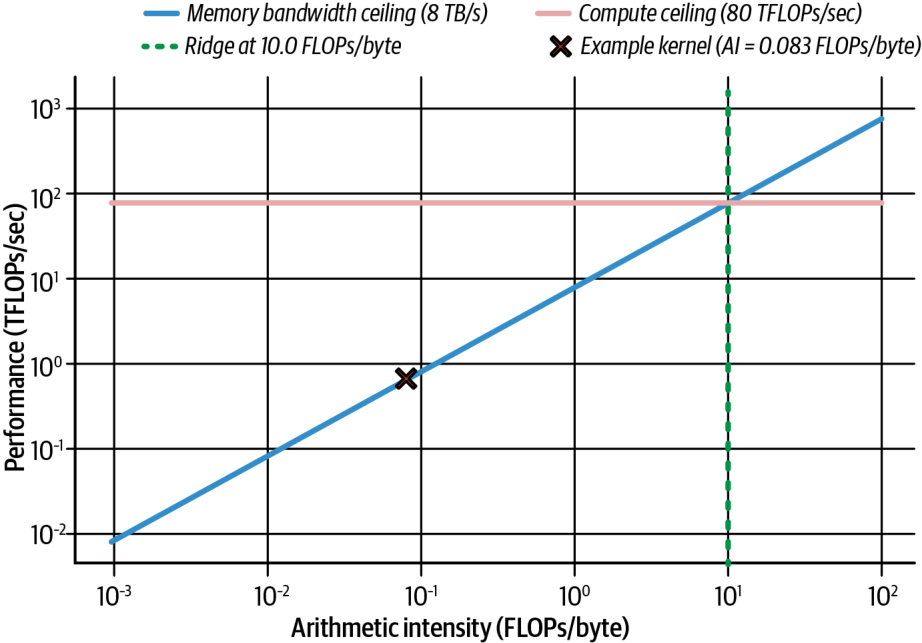
\includegraphics[width=\linewidth]{figs/fig6-21.png}\\
    {\scriptsize 图 6-21：Blackwell 级 GPU 的屋顶线；我们的 kernel 位于 0.083 FLOPs/字节}
  \end{columns}
  \medskip
  \pe{屋顶线先问一句：这个 kernel 是饿数学，还是饿数据？}\refmark{4}
\end{frame}

% ================================================================ 48
\begin{frame}{沿屋顶线向右走：低精度一鱼两吃}
  \begin{itemize}
    \item 想逃出内存受限区，就得\kw{让每个字节干更多活}：数据留在片上复用、
          算子融合 —— 或者干脆\kw{把字节变小}。
    \item 一次 128 字节的内存事务能装 \kw{32 个 FP32 = 64 个 FP16 = 128 个 FP8 = 256 个 FP4}。
          FP32 $\to$ FP16 立刻让 FLOPs/字节\kw{翻倍}；FP8 相对 FP16 又把吞吐翻倍、
          内存再省一半。
    \item Blackwell 原生支持 \kw{FP8 与 FP4 Tensor Core}，还有\kw{硬件解压}：
          权重以压缩形态存在 HBM 里（甚至比 FP4 更狠 —— 4 比特/2 比特方案），
          读取时即时展开，再转成 FP16/FP32 做精确累加。
    \item 净收益：\kw{等效内存带宽变大} —— 对内存受限的\kw{token 生成}
          是一项体系结构级的优势。
  \end{itemize}
  \medskip
  \begin{block}{要点}
    精度既是算力优化，更是\kw{带宽}优化：
    字节减半 $\Rightarrow$ 算术强度翻倍 $\Rightarrow$ 向算力屋顶靠近。
  \end{block}
\end{frame}

% ================================================================ 49
\begin{frame}{Profiling 工作流：诊断、修复、复测}
  \begin{columns}[c]
    \column{0.52\textwidth}
    \begin{itemize}\small
      \item \kw{ncu} 里内存受限的典型指纹：\kw{DRAM 利用率高 + ALU 利用率低}
            —— warp 都在等内存。同时留意\kw{全局加载效率}是否下滑。
      \item \kw{nsys} 时间线上 kernel 之间的空档 = GPU 在等数据传输。
      \item 期望重叠却看到"先拷贝、后计算"串行排队？两个惯犯：
            不小心用了\kw{默认流的隐式同步}，或者\kw{忘了用锁页内存} ——
            没有锁页内存，\texttt{cudaMemcpyAsync} \kw{无法}与 kernel 重叠。
      \item ncu 新特性：\kw{range replay}、源码关联、启动栈大小指标。
      \item 修好之后：空档消失，\kw{访存管道利用率}逼近峰值。
    \end{itemize}
    \column{0.45\textwidth}
    \centering
    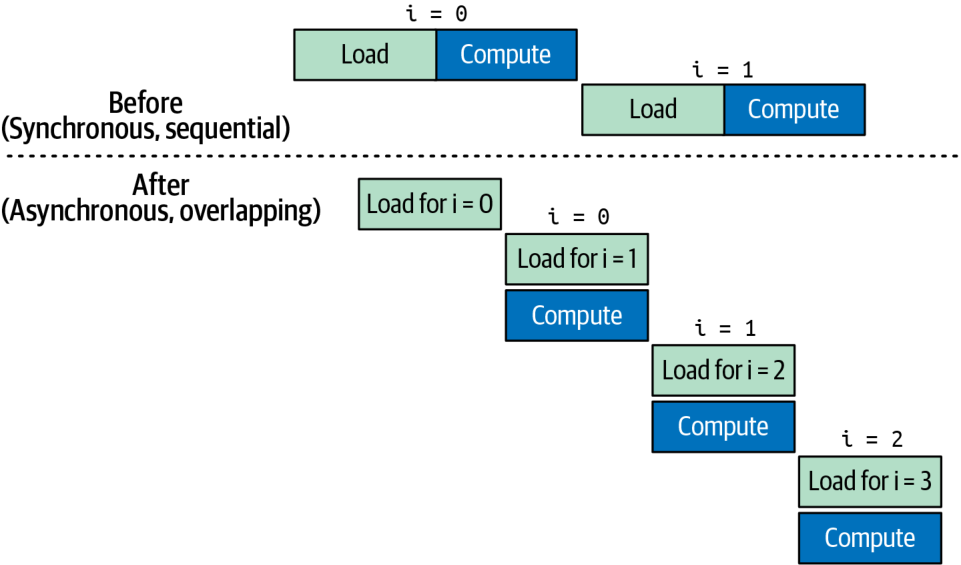
\includegraphics[width=\linewidth]{figs/fig6-22.png}\\
    {\scriptsize 图 6-22：同步（串行）vs.\ 异步（重叠）的传输 + 计算}
    \smallskip
    {\footnotesize\itshape 每改一处就测一次 —— 用 profiler 确认停顿真的减少了。}
  \end{columns}
\end{frame}

% ================================================================ 50
\begin{frame}{核心要点（书中的八条）}
  \begin{columns}[t]
    \column{0.48\textwidth}
    \begin{itemize}\small
      \item \kw{SIMT}：32 线程的 warp 齐步走；大量 warp 在飞 = 延迟被隐藏。
      \item \kw{层级}：线程 $\to$ block（$\leq$1{,}024）$\to$ grid；尽量少用
            \texttt{\_\_syncthreads()} 栅栏。
      \item \kw{占用率 vs.\ 上限}：取 32 的倍数；每 SM：64 warp、32 block、
            228 KB 共享内存、每线程 255 寄存器。
      \item \kw{启动参数}：先用 256 线程/block；网格 = ceil(N/256)；
            再用 profiler 调。
    \end{itemize}
    \column{0.48\textwidth}
    \begin{itemize}\small
      \item \kw{异步内存}：\texttt{cudaMallocAsync} + 流 + 内存池；
            PyTorch 的缓存分配器同理。
      \item \kw{内存阶梯}：在寄存器/共享内存/L1 里复用；对 L2/HBM 做合并访问。
      \item \kw{统一内存}：预取 + 建议，消灭突发停顿。
      \item \kw{屋顶线}：FLOPs/字节决定主战场；FP16/FP8/FP4 + 硬件解压帮你向右移动；
            \kw{TMEM + UMMA} 可以把 kernel 从内存受限拉成算力受限。
    \end{itemize}
  \end{columns}
\end{frame}

% ================================================================ 51
\begin{frame}{总结与下一步}
  \begin{block}{一句话总结本章}
    让 GPU \kw{忙起来}（占用率），让数据\kw{靠得近}（内存层级），
    让\kw{屋顶线}告诉你下一仗该打哪。
  \end{block}
  \begin{itemize}
    \item 书中的收尾提醒：\kw{最大占用率并不总是最优} ——
          单线程 \kw{ILP} 足够时，中低占用率也能赢；有时
          \kw{线程更少、每人寄存器更多}反而更快。\kw{一切以实测为准。}
    \item 本书接下来：warp 分化与访存调优（第 7--8 章）、
          算术强度（第 9 章）、TMA 与 warp 专业化（第 10 章）。
    \item 我的第二讲 —— \kw{第 12 章} —— 建立在本章之上：单个 kernel 快了之后，
          怎么\kw{编排}它们，让 GPU 永远不用等 CPU？
  \end{itemize}
  \medskip
  \centering\itshape 欢迎提问！
\end{frame}

% ================================================================ 52
\begin{frame}{参考文献与延伸阅读}
  {\footnotesize
  \begin{enumerate}
    \item C.\ Fregly. \emph{AI Systems Performance Engineering}（O'Reilly, 2026），第 6 章。
    \item NVIDIA. \emph{Blackwell Tuning Guide} 与 \emph{Blackwell Architecture Whitepaper} ——
          SM 上限、双发射调度器、TMEM 与 tcgen05。
    \item NVIDIA. \emph{CUDA C++ Programming Guide} —— 线程层级、统一内存、
          Occupancy API、\texttt{\_\_launch\_bounds\_\_}、流序内存分配、PTX/fatbin。
    \item S.\ Williams, A.\ Waterman, D.\ Patterson. \emph{Roofline: An Insightful Visual Performance
          Model for Multicore Architectures}. CACM 52(4), 2009.
    \item NVIDIA. \emph{Compute Sanitizer User Guide} —— memcheck、racecheck、initcheck、synccheck。
    \item NVIDIA. \emph{Nsight Systems} 与 \emph{Nsight Compute} 文档 —— NVTX、
          \texttt{nsys profile} 与 \texttt{ncu --section SpeedOfLight}。
    \item 本书代码与基准：本书 GitHub 仓库（本 deck 中示意表格的分架构真实数据）。
  \end{enumerate}}
\end{frame}

\end{document}
